\documentclass{article}
\usepackage{graphicx}
\usepackage[fleqn]{amsmath}
\usepackage[a4paper, margin=2cm]{geometry}
\newcommand{\comment}[1]{}
\begin{document}
\title{COS 214 Practical 1}
\author{Janco Spies, u21434159}
\maketitle
\section*{Task 1}
\begin{itemize}
    \item[1.1]\textbf{a}: Stack, since no dynamic memory has been allocated to the variable.\\
               \textbf{b}: Heap, since the new keyword indicates that dynamic memory was allocated to the variable.\\
               \textbf{c}: Stack, since no dynamic memory has been allocated to the variable.\\
               \textbf{n}: Stack, since no dynamic memory has been allocated to the variable.\\
               \textbf{d}: Stack, since no dynamic memory has been allocated to the variable.\\
               \textbf{e}: Stack, since no dynamic memory has been allocated to the variable.\\
               \textbf{f}: Stack, since no dynamic memory has been allocated to the variable.\\
               \textbf{g}: Stack, since no dynamic memory has been allocated to the variable.\\
               \textbf{h}: Stack, since no dynamic memory has been allocated to the variable.\\
               \textbf{c[10]}: Stack, since no dynamic memory has been allocated to the variable.
    \item[1.2] This would not work since NULL is not a valid value for an \textit{int} variable so the value zero will be stored there instead.
    \item[1.3] \textbf{void* f = (void*) 0xacfe2675;}\\ This line might not work since whatever value was stored at the memory address "0xacfe2675" cannot necessarily be cast to \textit{void*} which might lead to an error.\\~\\
                \textbf{c[10] = *\&*e;}\\ This line might not work since a \textit{char} array is being given the value of an \textit{int} pointer which does not have the same size.\\~\\
                \textbf{const int* e = (const int*) 522;}\\ This line might not work since e is a pointer pointing to a memory address of a literal, but this literal is not stored there in a variable so following this pointer will lead to a segmentation fault.
\end{itemize}

\section*{Task 2}
\begin{itemize}
    \item[2.1]The constructor for ClassA is called first for any class derived from ClassA.
    \item[2.2]The destructor for ClassA is called last for any class derived from ClassA. 
    \item[2.3]The constructor of ClassC is called after the constructor of ClassA.
    \item[2.4]ClassA then ClassB.
    \item[2.5]classB then ClassA. 
\end{itemize}

\section*{Task 3}
\begin{itemize}
    \item[3.2] 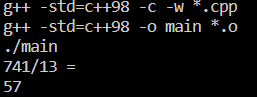
\includegraphics[width=0.25\textwidth]{../img/Task3_2.png}\\
                This worked since the calculator was instantiated with the \textit{int}
                datatype for which the division operator is defined.
    \item[3.3] 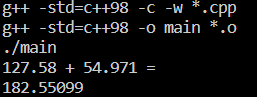
\includegraphics[width=0.25\textwidth]{../img/Task3_3.png}\\
                This worked since the calculator was instantiated with the \textit{double}
                datatype for which the addition operator is defined.
    \item[3.4] 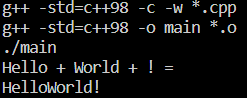
\includegraphics[width=0.25\textwidth]{../img/Task3_4.png}\\
                This worked since the calculator was instantiated with the \textit{string}
                datatype for which the addition operator is defined.
    \item[3.5] This does not work since the multiplication operator is not defined for 
                the \textit{string} datatype.
\end{itemize}

\section*{Task 4}
\begin{itemize}
    \item[4.1] \textbf{cout$<<$*ptr\_a$<<$"\_"$<<$*ptr\_b$<<$"\textbackslash n";} \\
                This line will output "15\_15" since the value ptr\_a points to is set to
                15 and ptr\_b is set to ptr\_a, which means that both pointers point to the value 15.
    \item[4.2] \textbf{cout$<<$*ptr\_a$<<$"\_"$<<$*ptr\_b$<<$"\textbackslash n";} \\
                This line will output "15\_4" since ptr\_a still points to 15 while 
                ptr\_b is set to point to a new value of 4.
    \item[4.3] \textbf{cout$<<$*ptr\_a$<<$"\_"$<<$*ptr\_b$<<$"\textbackslash n";} \\
                This line will output "15\_15" since ptr\_b's value that it points to
                is set to the same value that ptr\_a points to, which is 15.
    \item[4.4] \textbf{cout$<<$*ptr\_a$<<$"\_"$<<$*\&*\&*\&*\&*ptr\_b$<<$"\textbackslash n";} \\
                This line will output "15\_15" since after ptr\_a is deleted it is set 
                to ptr\_b which points to 15. The reference and dereference operators in 
                the cout statement cancel each other out until only the one dereference 
                operator is left.
    \item[4.5] \textbf{cout$<<$*ptr\_c$<<$"\_"$<<$**ptr\_c$<<$"\textbackslash n";} \\
                This line will output the address of ptr\_a followed by "\_15" since
                ptr\_c is set to the address of ptr\_a which in turn points to the value 15.
\end{itemize}

\section*{Task 5}
\begin{itemize}
    \item[5.2] My machine has a limited amount of memory which causes the program to run into 
    a segmentation fault after a certain amount of time when trying to compute such a large number,
     even though the implementation
     works for lesser values of m and n.\\
    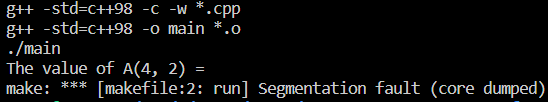
\includegraphics[width=0.6\textwidth]{../img/Task5_2.png}
\end{itemize}

\section*{Task 6}
\begin{itemize}
    \item[6.1] The \textbf{AuditableSnapshot} class is equivalent to the Memento interface. 
    \item[6.2] The \textbf{Snapshot} class is equivalent to the ConcreteMemento class. 
    \item[6.3] The \textbf{User} class is equivalent to the Originator class.
    \item[6.4] The \textbf{Store} class is equivalent to the Caretaker class.
    \item[6.7] 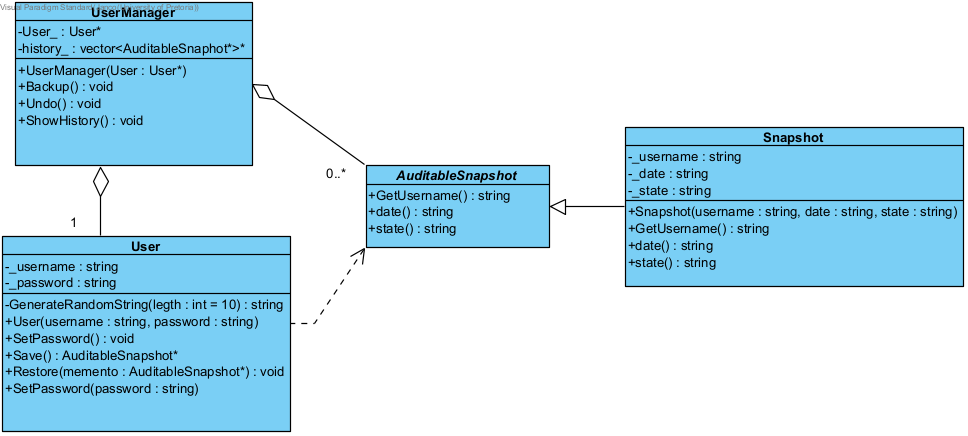
\includegraphics[width=0.7\textwidth]{../img/Task6_7.png}   
\end{itemize}
\end{document}